\documentclass[11pt,a4paper]{article}
\usepackage[margin=2.2cm]{geometry}
\usepackage{graphicx}
\usepackage{booktabs}
\usepackage{amsmath}
\usepackage{siunitx}
\usepackage{xcolor}
\usepackage{caption}
\usepackage{subcaption}
\usepackage{enumitem}
\usepackage[hidelinks]{hyperref}

\graphicspath{{../figures/}}
\setlist{nosep, leftmargin=*}
\captionsetup{font=small}
\emergencystretch=3em % lets lines with long \texttt paths break instead of overflowing

\title{ML-Driven PVT-Variation-Aware Leakage Estimation\\[2pt]
       \large Digital VLSI Design --- Course Project Report}
\author{%
  Gaurav Reddy Yerreddi (2024112006) \and
  Neel Rajesh (2024112007) \and
  Monishram Selvaraj (2024112076) \and
  Yogesh Krishna (2024102035)}
\date{}

\begin{document}
\maketitle

\section*{Summary}
Four MLP transistor models (NMOS/PMOS, ON/OFF), trained on 4 $\times$ 10{,}000 ngspice samples of the
\texttt{32nm\_HP.pm} card, predict the four terminal currents with a test-set median error of 0.14--0.15\,\%
for NMOS ON, NMOS OFF and PMOS ON and 8.4\,\% for PMOS OFF. Built from these models, the leakage of the
five gates (18 input cases $\times$ 200 PVT corners) has a median error of 1.40\,\% and a mean accuracy
(100\,\% minus the mean $|$error$|$) of 97.4\,\% against SPICE, and the 8-bit parity checker (28 NAND2,
256 input vectors $\times$ 200 corners) 1.36\,\% and 97.6\,\%, short of the 99\,\% target. At both levels
the error comes almost entirely from the drain current of OFF PMOS transistors, whose model is 15 times
less accurate than the NMOS OFF model even well above the simulator noise floor (1.8 against 0.12\,\%
for $|I_d| \ge \SI{1e-12}{A}$). With the OFF-PMOS-dominated gates replaced by their SPICE leakage, the
parity checker would reach 99.6\,\% mean accuracy, so the PMOS OFF model is the one thing that stands
between this method and the target.

\section{Introduction}
Leakage is a large part of the power of nanometre CMOS and depends exponentially on threshold voltage
and temperature~\cite{roy2003}, so estimating it across process, voltage and temperature (PVT) corners
needs many simulations. The project replaces those simulations by a three-level model: machine-learning
models of single transistors predict their terminal currents, gate leakage is assembled from the
transistor predictions, and circuit leakage from the gate predictions. Each level is checked against
ngspice~\cite{ngspice} with the PTM 32\,nm high-performance BSIM4 card~\cite{ptm,bsim4}.

\section{Setup}

\begin{table}[!htbp]
\centering
\begin{minipage}[t]{0.52\linewidth}
\centering
\caption{Assignment and simulator.}
\label{tab:setup}
\begin{tabular}{ll}
\toprule
Item & Value \\
\midrule
Model file      & \texttt{32nm\_HP.pm} (PTM BSIM4) \\
Channel length  & $L = L_{\min} = 32$\,nm \\
Nominal VDD     & 0.9\,V \\
Test circuit    & 8-bit parity checker \\
Simulator       & ngspice-47 \\
\bottomrule
\end{tabular}
\end{minipage}\hfill
\begin{minipage}[t]{0.46\linewidth}
\centering
\caption{Nominal process parameters.}
\label{tab:nominal}
\begin{tabular}{lcc}
\toprule
Parameter & NMOS & PMOS \\
\midrule
$v_{th0}$ (V)                  & 0.49396 & $-0.49155$ \\
$t_{oxe}$ (nm)                 & 1.15 & 1.20 \\
$n_{dep}$ (cm$^{-3}$)          & $4.12\times10^{18}$ & $3.07\times10^{18}$ \\
$u_0$ (m$^2$/V\,s)             & 0.050 & 0.014 \\
$x_j$ (nm)                     & 10 & 10 \\
\bottomrule
\end{tabular}
\end{minipage}
\end{table}

The nominal values in Table~\ref{tab:nominal} are read from the model card. Models were trained
with Python 3.11, PyTorch 2.15~\cite{pytorch} and scikit-learn 1.9~\cite{sklearn} on CPU. All scripts
read the assignment, sampling ranges and seeds from a single \texttt{config.yaml} and run in numeric
order (\texttt{01} to \texttt{09}).

\section{Data generation}

\subsection{Sampling}
For each of the four cases (NMOS ON, NMOS OFF, PMOS ON, PMOS OFF), 10,000 samples were drawn
independently (seed 2026, one random stream per case), following Section~4 of the project spec:
\begin{itemize}
  \item $V_{DD} \sim U(0.81, 0.99)$\,V, drawn first; then $V_d, V_s \sim U(0, V_{DD})$;
  \item $W \sim U(1, 8)\cdot L_{\min}$; $T \sim U(-40, 125)$\,\si{\celsius};
  \item $v_{th0}, t_{oxe}, n_{dep}, u_0, x_j$ each $= \text{nominal}\times U(0.9, 1.1)$, drawn separately for NMOS and PMOS;
  \item $V_g, V_b$ fixed by the case (NMOS ON: $V_{DD}, 0$; NMOS OFF: $0, 0$; PMOS ON: $0, V_{DD}$; PMOS OFF: $V_{DD}, V_{DD}$).
\end{itemize}
Each dataset is stored as one CSV with columns
\texttt{vdd, temp, w, vd, vs, vg, vb, vth0, toxe, ndep, u0, xj, id, ig, is, ib} (SI units).
The spec's 10,000 samples per case were kept. For three cases the test error is already about
0.15\,\%, and for PMOS OFF the error is not set by the number of samples (Section~\ref{sec:errors});
a learning curve to find the smallest sufficient dataset was not run (Section~\ref{sec:limits}).

\subsection{Netlists}
Each case has a hand-written single-transistor netlist (\texttt{netlists/transistor/<case>.cir})
that runs on its own with \texttt{ngspice -b}. Every terminal has its own DC voltage source, and
each netlist contains the required
\texttt{.options gmin=1e-18 abstol=1e-18 reltol=1e-6 vntol=1e-9}.
The generation script replaces the \texttt{.param} values with each sample and runs ngspice
once per sample (about 2 minutes for all 40,000 runs, 8 parallel processes).
\begin{itemize}
  \item \textbf{Process parameters} are applied with \texttt{altermod}, one line per parameter:
        a multi-parameter \texttt{altermod} line in ngspice silently applies only the first one.
        A sensitivity test confirmed that all five parameters reach the simulator.
  \item \textbf{Junction geometry:} $AD = AS = W L_{\mathrm{diff}}$, $PD = PS = 2(W + L_{\mathrm{diff}})$ with
        $L_{\mathrm{diff}} = 2L_{\min}$, as specified by the TAs. Only $I_b$ depends on it.
  \item \textbf{Sign convention:} every stored current flows \emph{into} the device terminal
        ($I = -\,\texttt{i(Vsource)}$); \texttt{set numdgt=12} keeps the printed currents from being
        rounded to 6 digits.
\end{itemize}

\subsection{Train / validation / test split}
Each dataset was split 70/15/15 (7,000 / 1,500 / 1,500 rows) with a fixed seed (42). The split
is stored as a file per case and shared by all four model types, so every model is trained,
tuned and tested on exactly the same rows. Tuning used the validation set only; the test set is
used only for the chosen models.

\subsection{Data check}\label{sec:kcl}
\paragraph{Kirchhoff check.} Table~\ref{tab:kcl} lists $|I_d + I_g + I_s + I_b|$ per case.
The residual of about \SI{1e-16}{A} comes from the gate and substrate resistance networks
enabled in the PTM card (\texttt{rgatemod=1}, \texttt{rbodymod=1}); with both switched off the
residual drops to \SI{1e-31}{A}. The model card was used unmodified. The practical consequence
is a simulator noise floor: currents below about \SI{1e-15}{A} are not reproducible between
equivalent simulations. This affects mainly PMOS OFF $I_g$ (62\,\% of rows), PMOS OFF and NMOS OFF
$I_b$ (54\,\%), and about 20\,\% of PMOS OFF $I_d/I_s$.

\begin{table}[!htbp]
\centering
\caption{Kirchhoff check: $|I_d+I_g+I_s+I_b|$ over the 10,000 samples of each case.}
\label{tab:kcl}
\begin{tabular}{lcc}
\toprule
Case & Median (A) & Max (A) \\
\midrule
NMOS ON  & \num{9.1e-17} & \num{1.2e-15} \\
NMOS OFF & \num{2.0e-23} & \num{5.1e-20} \\
PMOS ON  & \num{3.0e-17} & \num{6.0e-16} \\
PMOS OFF & \num{7.7e-17} & \num{1.0e-15} \\
\bottomrule
\end{tabular}
\end{table}

\paragraph{Trend plots.} Figure~\ref{fig:trends} shows the raw dataset values. OFF current
($|I_d|$ of the OFF datasets) rises by several decades from $-40$ to \SI{125}{\celsius}
(subthreshold slope and $V_{th}$ fall with temperature). Gate current falls steeply with $t_{oxe}$,
as expected for direct tunnelling. OFF current also falls with $|v_{th0}|$, but this trend is
weaker in the raw scatter: a $\pm10\,\%$ change in $v_{th0}$ moves $I_{\mathrm{off}}$ less than the spread
caused by the other random inputs ($T$, $W$, $V_d$, $V_s$). The PMOS OFF data also show a narrow lower
branch: samples with both $V_d$ and $V_s$ far below VDD (median 0.4\,V), where the channel is deeply off
and $|I_d|$ is consistent with drain-junction leakage, which rises with temperature and falls into the
noise floor below about \SI{50}{\celsius}.

\begin{figure}[!htbp]
\centering
\begin{subfigure}{0.49\linewidth}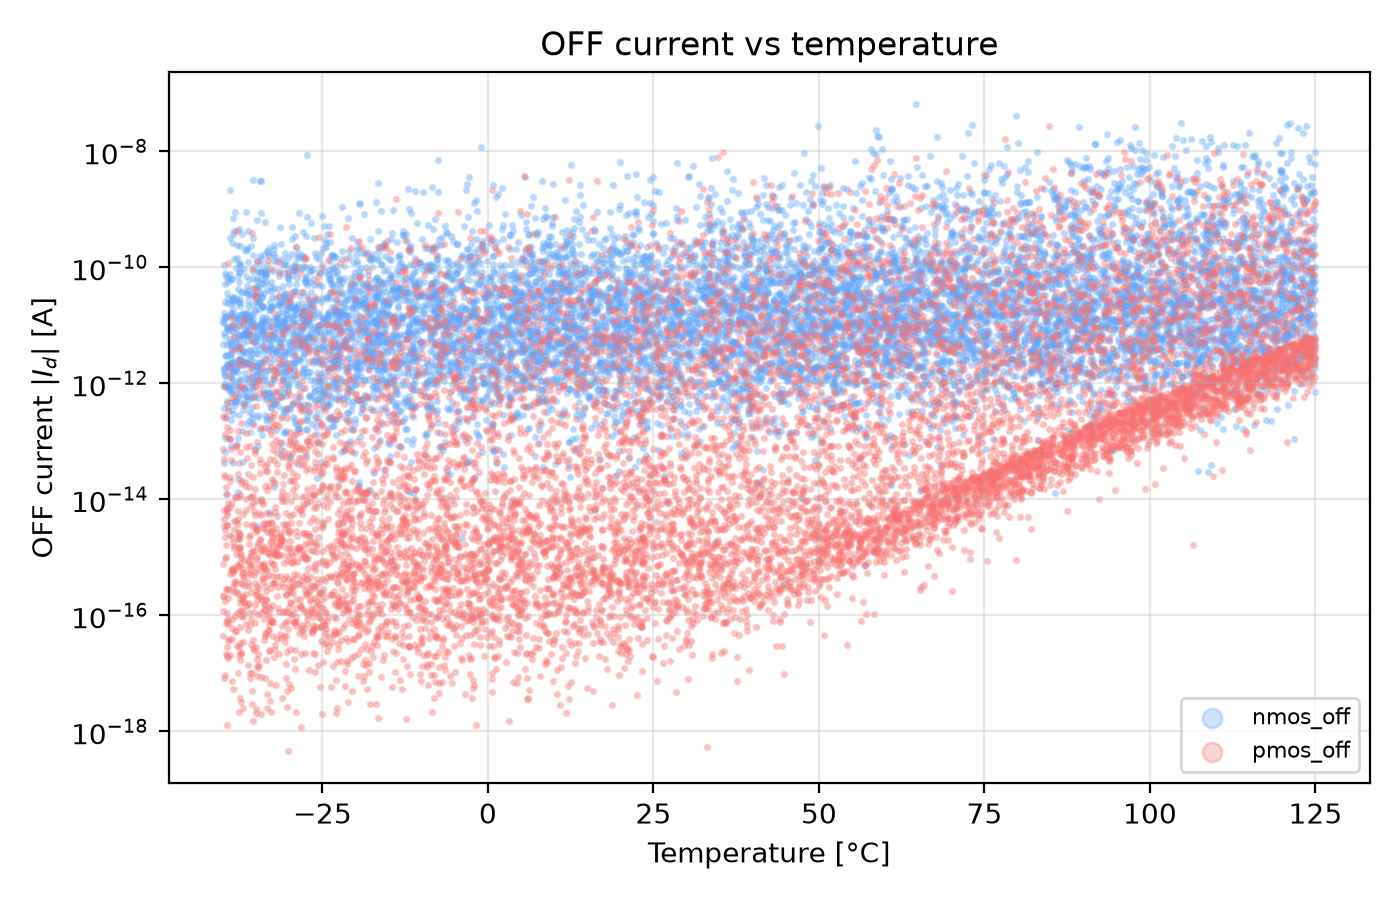
\includegraphics[width=\linewidth]{trend_ioff_vs_temp.png}\caption{$I_{\mathrm{off}}$ vs $T$}\end{subfigure}
\begin{subfigure}{0.49\linewidth}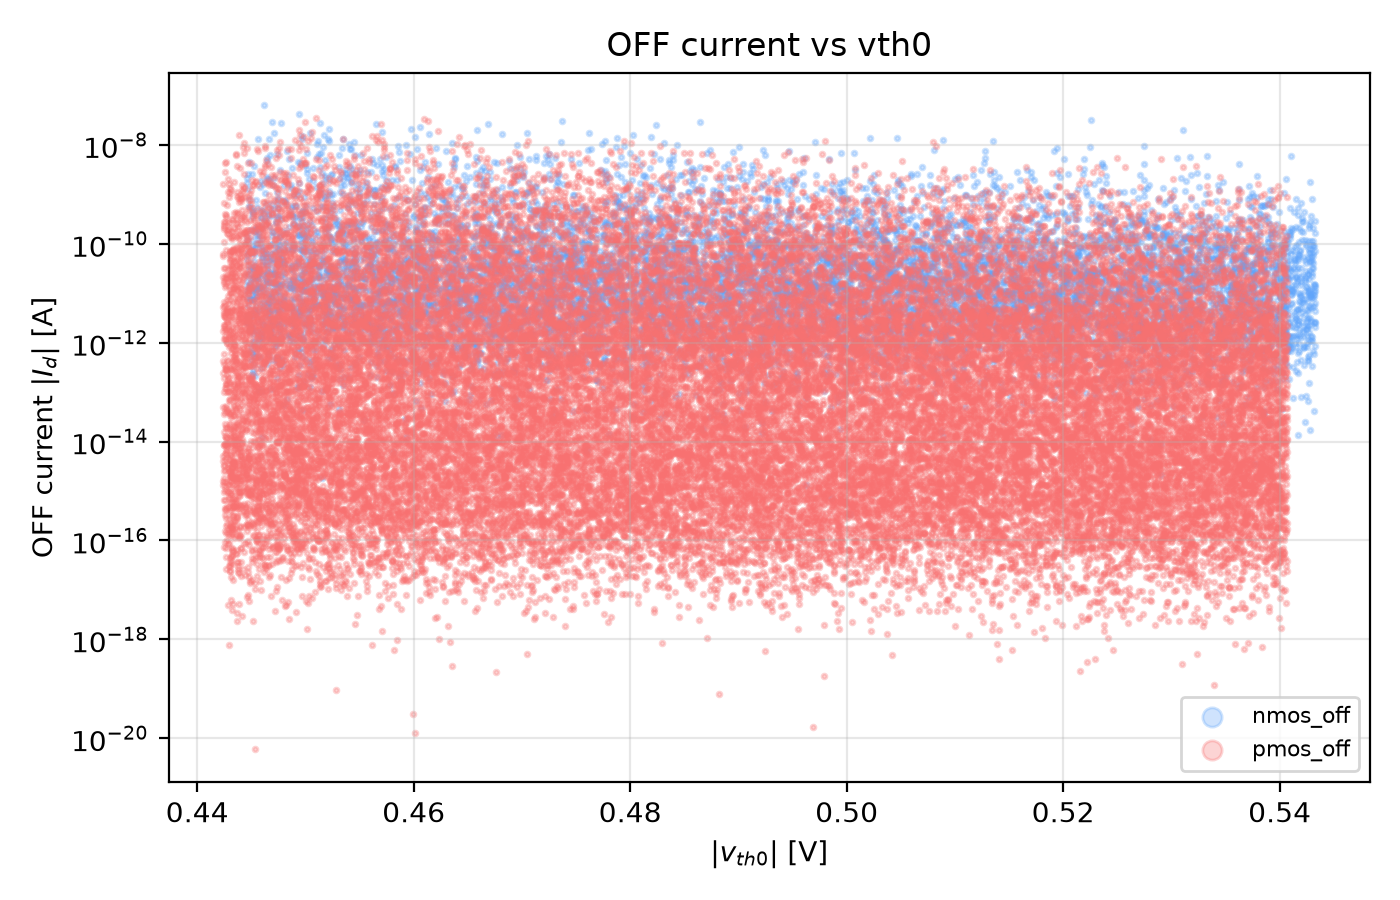
\includegraphics[width=\linewidth]{trend_ioff_vs_vth0.png}\caption{$I_{\mathrm{off}}$ vs $|v_{th0}|$}\end{subfigure}\\[4pt]
\begin{subfigure}{0.49\linewidth}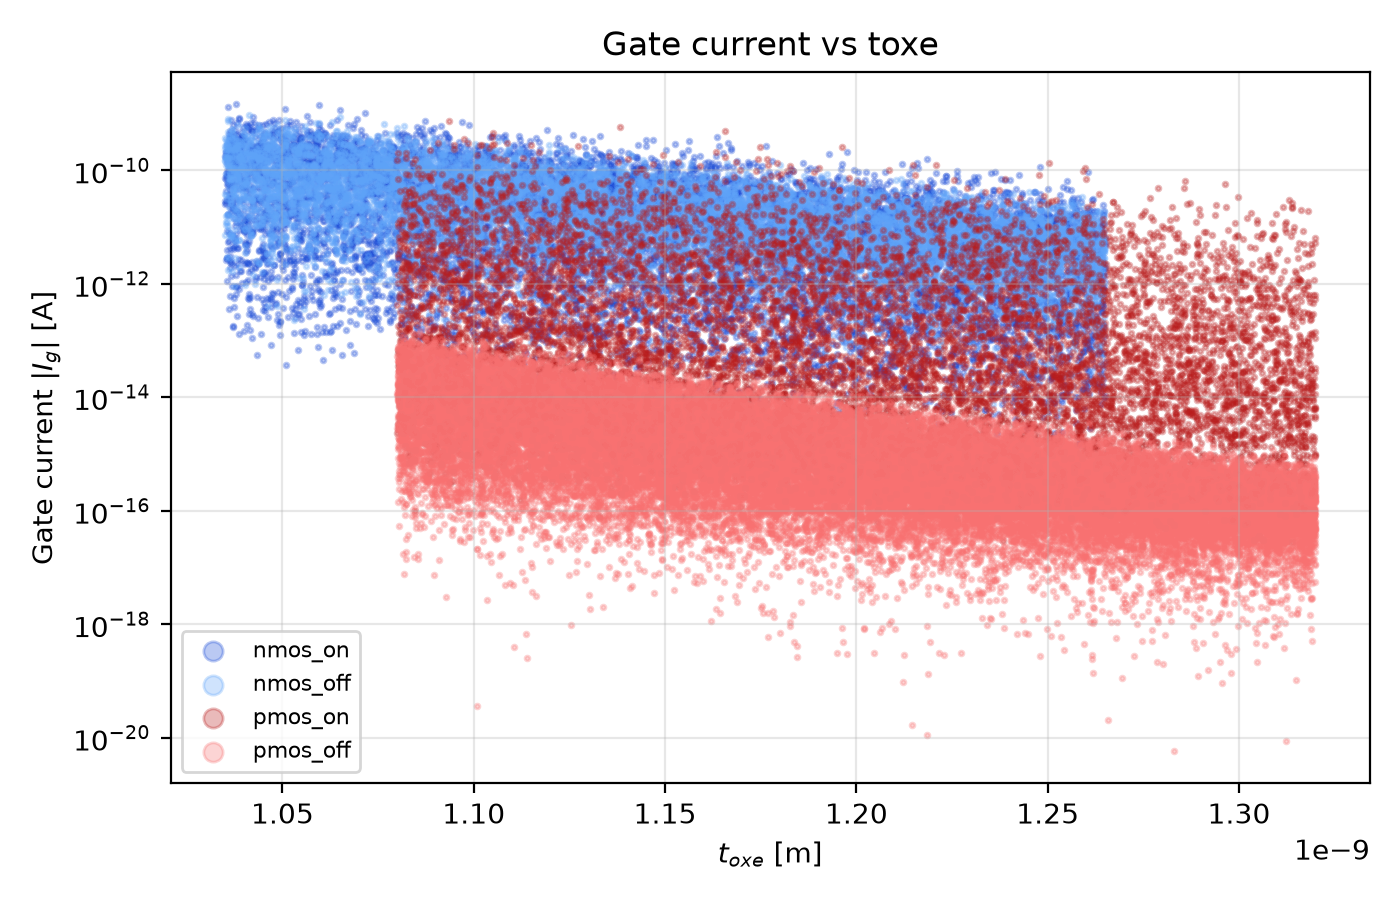
\includegraphics[width=\linewidth]{trend_ig_vs_toxe.png}\caption{$|I_g|$ vs $t_{oxe}$}\end{subfigure}
\caption{Data-check trend plots (NMOS and PMOS in different colours).}
\label{fig:trends}
\end{figure}

\section{Models}

\subsection{Common preprocessing and metrics}
All four model types are trained on the same training split and scored on the same validation
split with the same metrics; each chooses its own target scale, but every prediction is converted
back to amperes before scoring.
\begin{itemize}
  \item \textbf{Error:} relative error $|I_{\mathrm{pred}}-I_{\mathrm{SPICE}}|/|I_{\mathrm{SPICE}}|\times100\,\%$, reported as
        the median and 95th percentile per current, on all rows (noise-floor currents included).
  \item \textbf{$R^2$} is computed on the sign-preserving log scale $\operatorname{asinh}(I/\SI{1e-18}{A})$, since
        currents span 6--13 decades and about half of $I_d/I_s$ in the ON cases are negative. On such a
        scale even mediocre fits score above 0.99, so models are compared on the median and p95 error
        (Section~\ref{sec:choice}); $R^2$ is a secondary check.
\end{itemize}

\subsection{Model types}
\paragraph{MLP (PyTorch, chosen for all four cases).} One network per case predicts all four currents.
\emph{Targets.} Drain and source are first put in a canonical order: NMOS rows with $V_d < V_s$
and PMOS rows with $V_s < V_d$ have $V_d/V_s$ and $I_d/I_s$ swapped, and the predictions are swapped
back, so the canonical $I_d$ always flows in the channel direction and its sign is fixed. The network
predicts $\log_{10}(|I|/W)$ of each current, standardised, plus a sign output (logistic loss) for every
current whose sign is not fixed. The canonical $I_s$ keeps its sign output: in the OFF cases it is a
near-cancellation of channel and junction leakage and opposite to the channel direction in 59\,\% of
NMOS OFF and 44\,\% of PMOS OFF samples. Per case (chosen on the validation set, Appendix~\ref{app:tt}):
the ON cases also divide $I_d$ and $I_s$ by the subthreshold drain factor, target
$\log_{10}\bigl(|I| / (W(1-e^{-|V_{ds}|/V_T}))\bigr)$; the OFF cases add four inputs
($V_{ds}/V_T$, $V_{gs}/V_T$, $V_{bs}/V_T$, $\log_{10}(1-e^{-|V_{ds}|/V_T}+10^{-12})$, $V_T = kT/q$);
NMOS OFF takes $I_s = -(I_d + I_g + I_b)$ instead of predicting it; PMOS OFF trains on labels clipped
to $|I| \ge \SI{1e-17}{A}$ (it is still scored against the raw SPICE values).
\emph{Inputs:} the 12 CSV inputs plus $V_d-V_s$, $V_g-V_s$, $V_b-V_s$ and $1/T$, computed after the
swap and standardised on the training set.
\emph{Network:} fully connected, SiLU, L1 loss on the magnitudes, AdamW, one-cycle learning-rate
schedule (peak $3\times10^{-3}$), batch 256, seed 42. ON cases: $128\times3$, 6,000 epochs, no weight
decay; OFF cases: $256\times4$, 3,000 epochs, weight decay $10^{-3}$. These settings come from a
two-round validation search (Appendix~\ref{app:mlp}): L1 loss clearly beat MSE and Huber, SiLU beat
tanh and GELU. A first scikit-learn \texttt{MLPRegressor} underfit (6--7\,\% median error).

\paragraph{Polynomial ridge regression (scikit-learn).} Polynomial ridge fits on a log scale of three
sign-consistent quantities, $D/V_{ds}$ with $D = I_d - I_s$, $I_g$ and $I_b$, from which $I_d$ and $I_s$
follow and satisfy Kirchhoff exactly. Its 20 features are built in a drain/source-symmetric frame and
include physics-based terms (subthreshold drain factor, EKV inversion charges~\cite{ekv} at each channel
end, tunnelling and junction terms). Degree (2--4), $\alpha$ and the junction features were chosen per
part by the validation RMSE of the log target. Details in Appendix~\ref{app:models}.

\paragraph{Gradient-boosted trees (XGBoost~\cite{xgboost}).} Four boosters per case predict the channel
and common-mode parts of $I_d$/$I_s$, $I_g$ and $I_b$ on the asinh scale (normalised by $W$), from 31
symmetric, physics-based features, each starting from a least-squares baseline. 6,000 rounds, learning
rate 0.015, depth 6, subsampling 0.8; PMOS OFF uses an absolute-error (L1) loss because squared error
averages its noisy, mixed-sign $I_g$/$I_b$ labels towards zero. Details in Appendix~\ref{app:models}.

\paragraph{Random forest (scikit-learn).} One multi-output forest per case on the asinh scale, with 11
inputs (terminal-relative voltages and the process parameters) and four hyperparameters tuned one at a
time on validation $R^2$ (Appendix~\ref{app:models}). Its median errors are 35--91\,\%: a forest
predicts a piecewise-constant average of training labels and cannot follow currents that change
exponentially with voltage.

\subsection{Model comparison (validation set)}
Table~\ref{tab:cmp} gives the median error, p95 error and $R^2$ for each current, in the order
$I_d / I_g / I_s / I_b$.

\begin{table}[!htbp]
\centering
\footnotesize
\caption{Validation-set comparison (4 model types $\times$ 4 cases, 1{,}500 validation samples per
case). Errors in \%; $R^2$ on the $\operatorname{asinh}(I/\SI{1e-18}{A})$ scale. Each cell:
$I_d / I_g / I_s / I_b$. Source: \texttt{results/model\_comparison.csv}.}
\label{tab:cmp}
\setlength{\tabcolsep}{2.5pt}
\begin{tabular}{llccc}
\toprule
Model & Case & Median error (\%) & p95 error (\%) & $R^2$ \\
\midrule
MLP         & NMOS ON  & 0.12 / 0.16 / 0.12 / 0.22 & 0.9 / 1.6 / 0.9 / 1.2 & .9997 / 1.000 / .9996 / 1.000 \\
            & NMOS OFF & 0.13 / 0.06 / 0.13 / 0.21 & 1.6 / 0.4 / 1.4 / 1.3 & 1.000 / 1.000 / 1.000 / 1.000 \\
            & PMOS ON  & 0.13 / 0.12 / 0.14 / 0.23 & 0.7 / 0.5 / 0.7 / 3.2 & .9994 / 1.000 / 1.000 / .9999 \\
            & PMOS OFF & 3.17 / 14.29 / 3.08 / 11.98 & 24.3 / 332.2 / 22.5 / 510.4 & .9907 / .2043 / .9982 / .7354 \\
\midrule
XGBoost     & NMOS ON  & 3.38 / 0.94 / 3.38 / 5.67 & 17.1 / 5.9 / 17.1 / 19.0 & .9992 / .9997 / .9989 / .9989 \\
            & NMOS OFF & 2.93 / 0.36 / 3.07 / 1.63 & 32.8 / 1.5 / 36.6 / 17.9 & .9671 / .9999 / .9610 / .9998 \\
            & PMOS ON  & 3.43 / 2.06 / 3.43 / 6.04 & 15.1 / 9.0 / 15.3 / 22.0 & .9993 / .9997 / 1.000 / .9986 \\
            & PMOS OFF & 6.58 / 16.72 / 6.22 / 13.53 & 43.8 / 167.4 / 42.5 / 175.6 & .9941 / .4846 / .9969 / .8495 \\
\midrule
Poly. ridge & NMOS ON  & 0.32 / 2.00 / 0.32 / 5.13 & 1.8 / 14.2 / 1.8 / 18.7 & .9997 / .9988 / 1.000 / .9989 \\
            & NMOS OFF & 3.61 / 0.10 / 3.98 / 8.71 & 54.6 / 0.7 / 52.1 / 30.5 & .9540 / 1.000 / .9742 / .9994 \\
            & PMOS ON  & 0.20 / 0.18 / 0.20 / 6.81 & 0.8 / 1.0 / 0.8 / 21.6 & 1.000 / 1.000 / 1.000 / .9984 \\
            & PMOS OFF & 14.75 / 22.15 / 14.96 / 29.90 & 139.0 / 267.7 / 140.4 / 449.7 & .9849 / .3993 / .9884 / .6963 \\
\midrule
Random      & NMOS ON  & 44.30 / 73.76 / 44.19 / 53.61 & 286.5 / 710.3 / 281.1 / 365.6 & .9989 / .7372 / .9987 / .9069 \\
forest      & NMOS OFF & 76.32 / 77.25 / 73.10 / 34.98 & 419.7 / 700.2 / 527.1 / 164.8 & .9366 / .4426 / .9530 / .9891 \\
            & PMOS ON  & 48.01 / 67.45 / 48.05 / 55.04 & 302.7 / 567.8 / 311.4 / 368.9 & .9989 / .8753 / .9992 / .9072 \\
            & PMOS OFF & 73.86 / 90.78 / 74.37 / 83.24 & 479.6 / 642.2 / 739.6 / 155.8 & .9419 / .1976 / .9603 / .8584 \\
\bottomrule
\end{tabular}
\end{table}

\subsection{Final choice and test-set results}\label{sec:choice}
\textbf{Rule.} For each case, the chosen model type is the one with the lowest validation median
error averaged over $I_d, I_g, I_s, I_b$; the averaged p95 error is checked next to it. Only the
validation set is used for the choice; the test set is used afterwards, on the chosen models only.

\textbf{Choice} (validation, mean of the four medians / mean of the four p95):
\begin{itemize}
  \item \textbf{NMOS ON, NMOS OFF, PMOS ON: MLP} (0.15 / 1.1\,\%, 0.13 / 1.2\,\%, 0.15 / 1.3\,\%). Its median
        error is 12--15 times lower than the next model's, and its p95 is also the lowest.
  \item \textbf{PMOS OFF: MLP} (8.1 / 222\,\%, against 10.8 / 107\,\% for XGBoost). On $I_d$ and $I_s$, the
        currents that carry the gate leakage, the MLP is twice as accurate (median 3.2 / 3.1\,\% against
        6.6 / 6.2\,\%, p95 24 / 23\,\% against 44 / 43\,\%). The p95 check goes the other way only because
        of $I_g$ and $I_b$, of which about 60\,\% and 50\,\% lie below \SI{1e-15}{A}, at the simulator
        noise floor (Section~\ref{sec:kcl}), where their sign is close to random. The MLP is kept,
        following the rule.
\end{itemize}
The four chosen models are \texttt{saved\_models/mlp/<case>.joblib} (\texttt{results/chosen\_models.csv});
before the test run, each saved file is checked to reproduce its validation errors.

\begin{table}[!htbp]
\centering
\footnotesize
\caption{Chosen models on the test set (1{,}500 samples per case, not used for training or choice).
Errors in \%; each cell $I_d / I_g / I_s / I_b$, then the mean of the four.
Source: \texttt{results/test\_results.csv}.}
\label{tab:test}
\setlength{\tabcolsep}{4pt}
\begin{tabular}{llcccc}
\toprule
Case & Model & Median error (\%) & mean & p95 error (\%) & mean \\
\midrule
NMOS ON  & MLP & 0.13 / 0.14 / 0.13 / 0.21 & 0.15 & 0.8 / 1.4 / 0.8 / 1.2 & 1.1 \\
NMOS OFF & MLP & 0.14 / 0.06 / 0.13 / 0.22 & 0.14 & 1.5 / 0.4 / 1.8 / 1.5 & 1.3 \\
PMOS ON  & MLP & 0.13 / 0.11 / 0.13 / 0.21 & 0.14 & 0.7 / 0.6 / 0.7 / 4.1 & 1.5 \\
PMOS OFF & MLP & 3.01 / 15.77 / 2.99 / 11.90 & 8.42 & 23.3 / 450.0 / 25.7 / 621.0 & 280.0 \\
\bottomrule
\end{tabular}
\end{table}

The test errors are close to the validation errors (mean median 0.15 vs 0.15\,\%, 0.14 vs 0.13\,\%,
0.14 vs 0.15\,\% and 8.4 vs 8.1\,\%), so the choices made on the validation set did not overfit it.
Figures~\ref{fig:testplots_n} and~\ref{fig:testplots_p} plot predicted against SPICE currents on the
test set. In the ON cases no prediction has the wrong sign or an error above 100\,\%. For PMOS OFF,
476 of the 478 wrong-sign predictions (mostly $I_g$ and $I_b$) are at SPICE currents below about
\SI{1.3e-15}{A}, i.e.\ at the noise floor.

\begin{figure}[!htbp]
\centering
\begin{subfigure}{0.6\linewidth}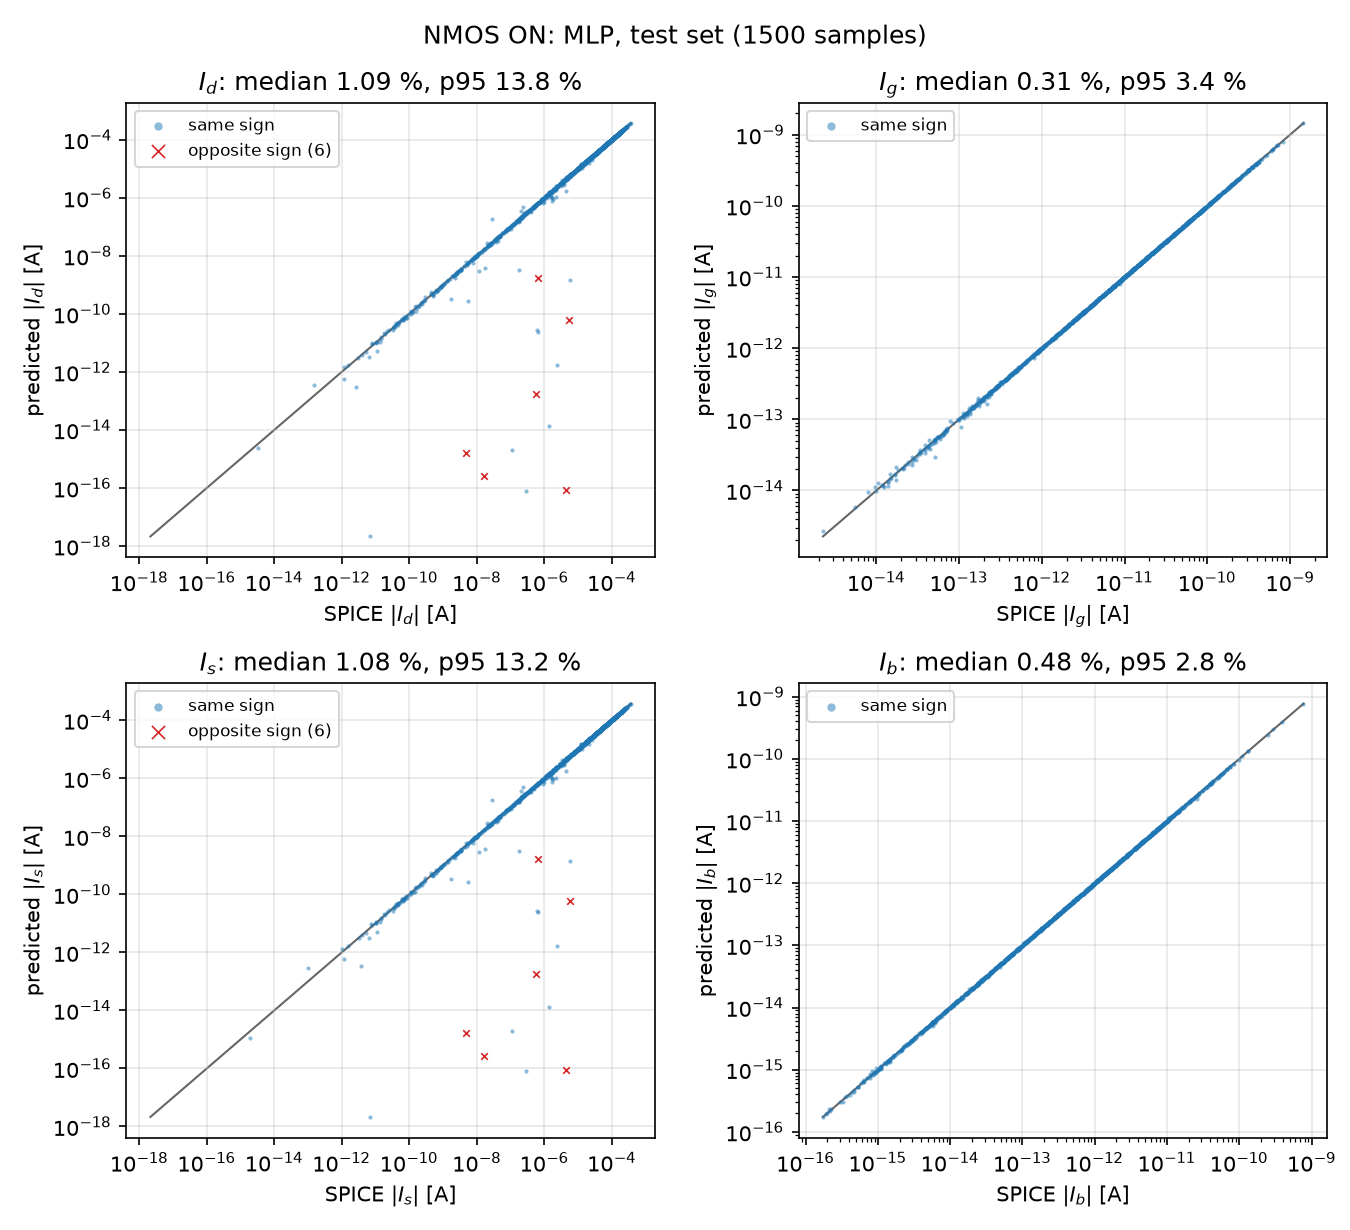
\includegraphics[width=\linewidth]{test_pred_vs_spice_nmos_on.png}\caption{NMOS ON}\end{subfigure}\\[4pt]
\begin{subfigure}{0.6\linewidth}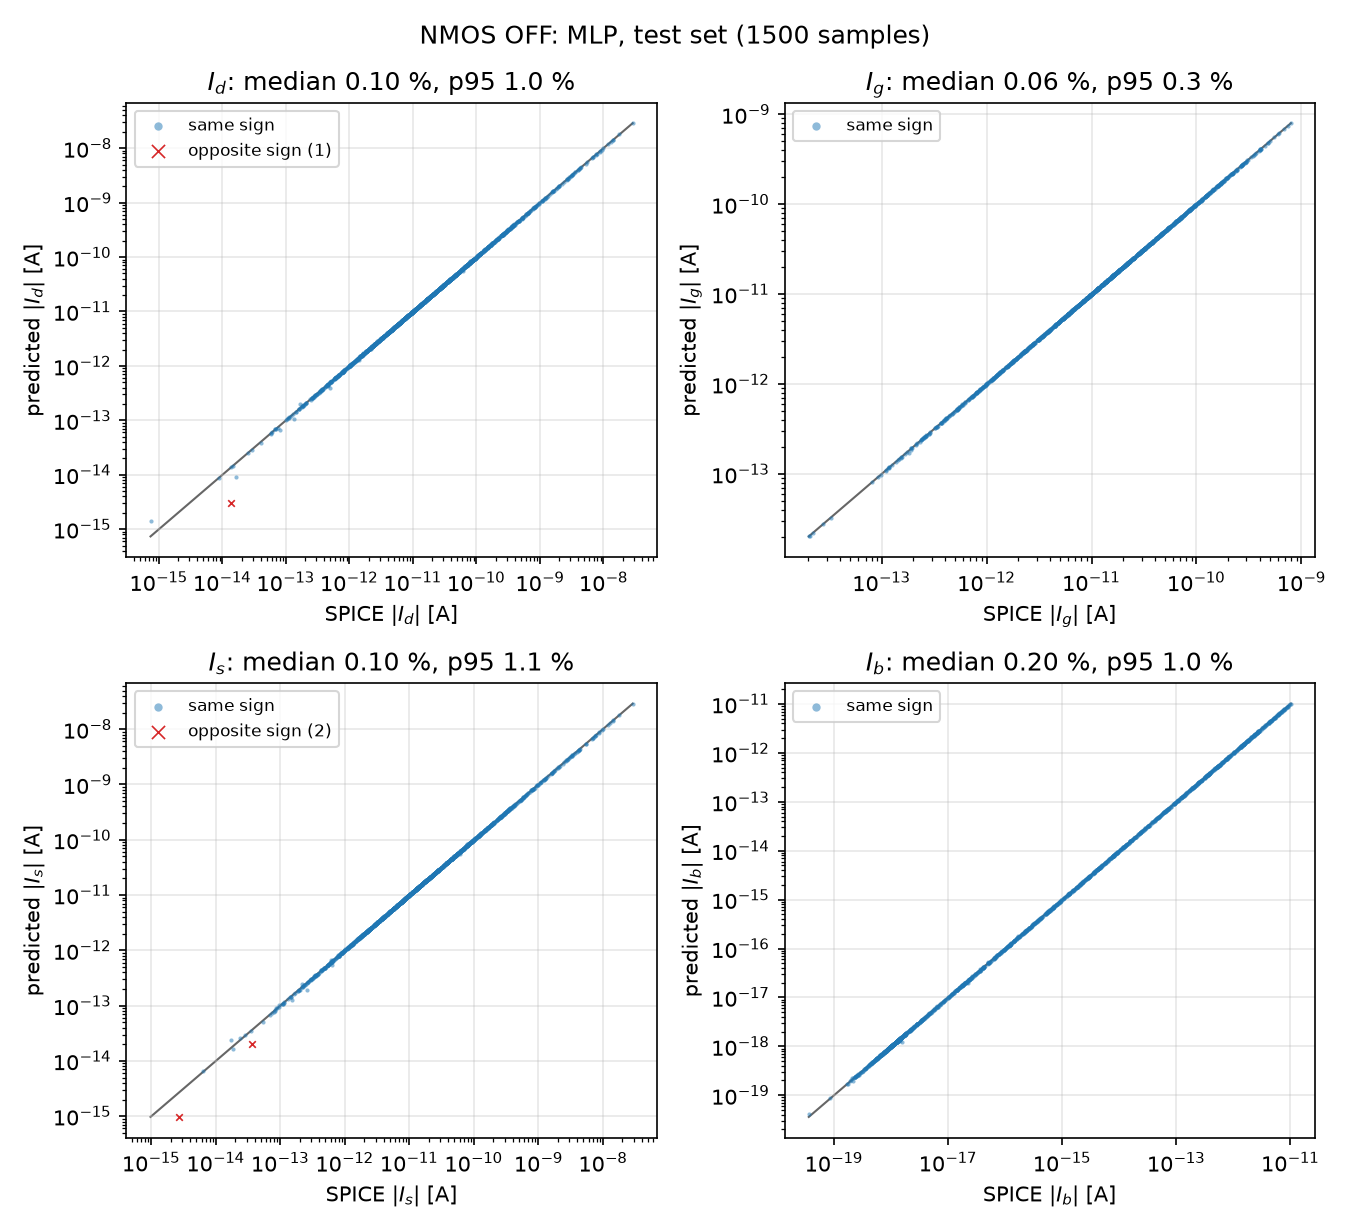
\includegraphics[width=\linewidth]{test_pred_vs_spice_nmos_off.png}\caption{NMOS OFF}\end{subfigure}
\caption{Predicted vs SPICE terminal currents of the chosen NMOS models (MLP) on the test set, $|I|$ on
log axes; red crosses: predicted sign opposite to SPICE.}
\label{fig:testplots_n}
\end{figure}

\begin{figure}[!htbp]
\centering
\begin{subfigure}{0.6\linewidth}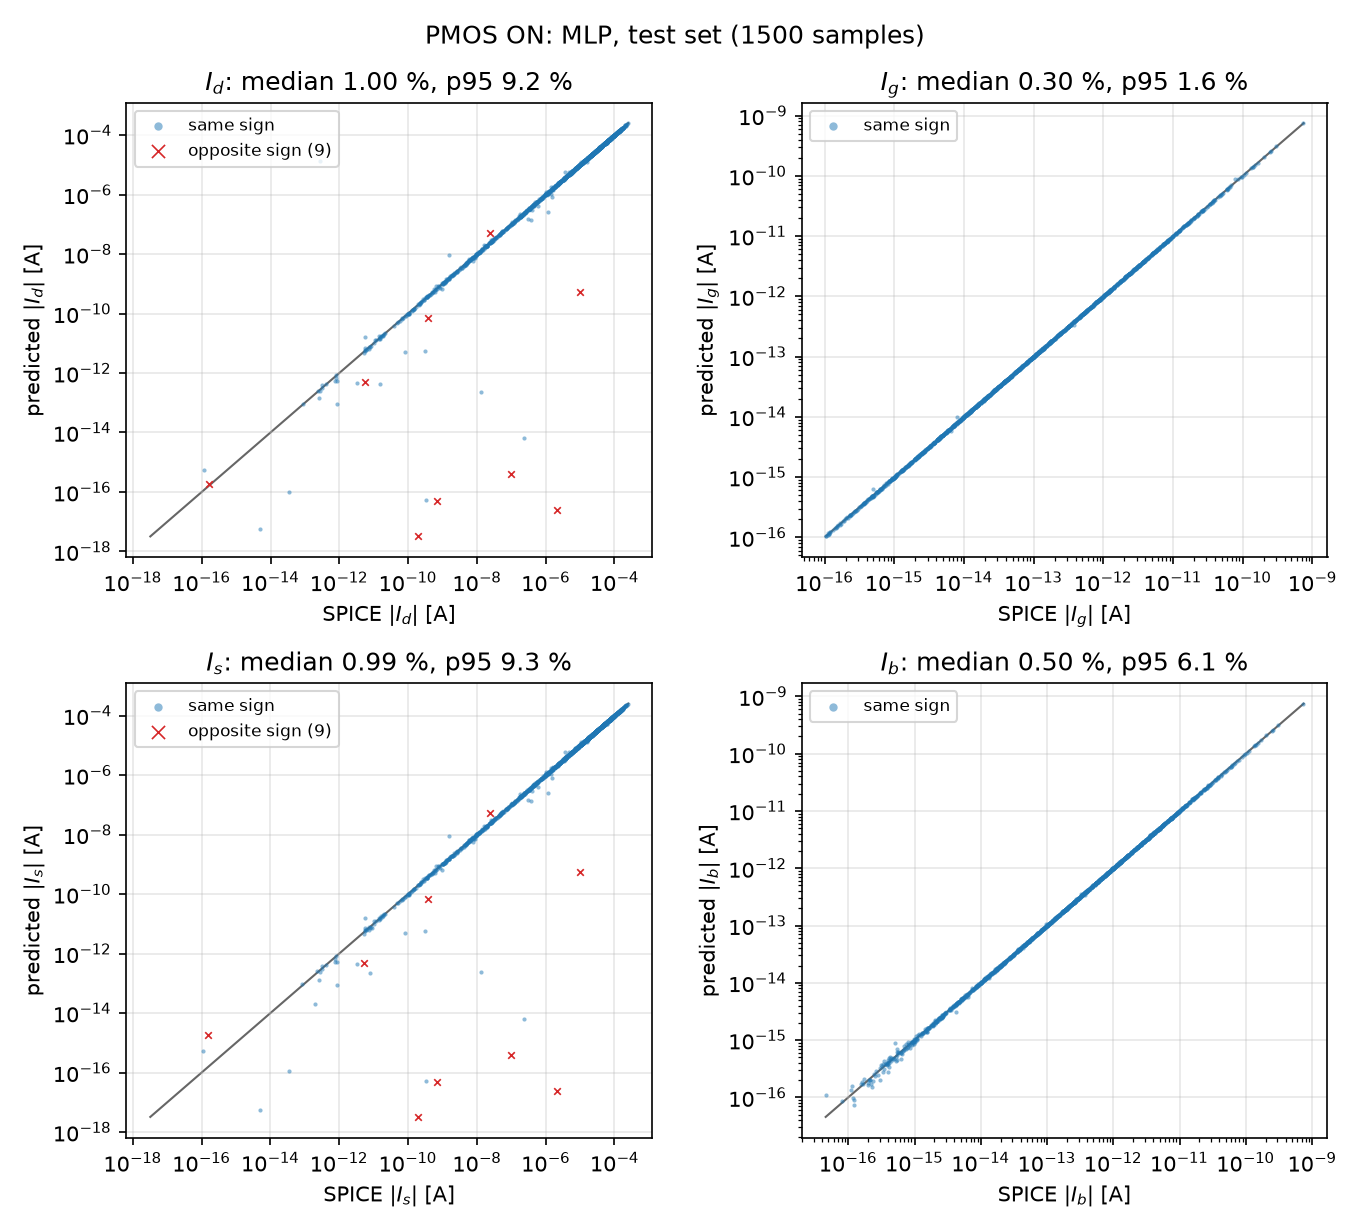
\includegraphics[width=\linewidth]{test_pred_vs_spice_pmos_on.png}\caption{PMOS ON}\end{subfigure}\\[4pt]
\begin{subfigure}{0.6\linewidth}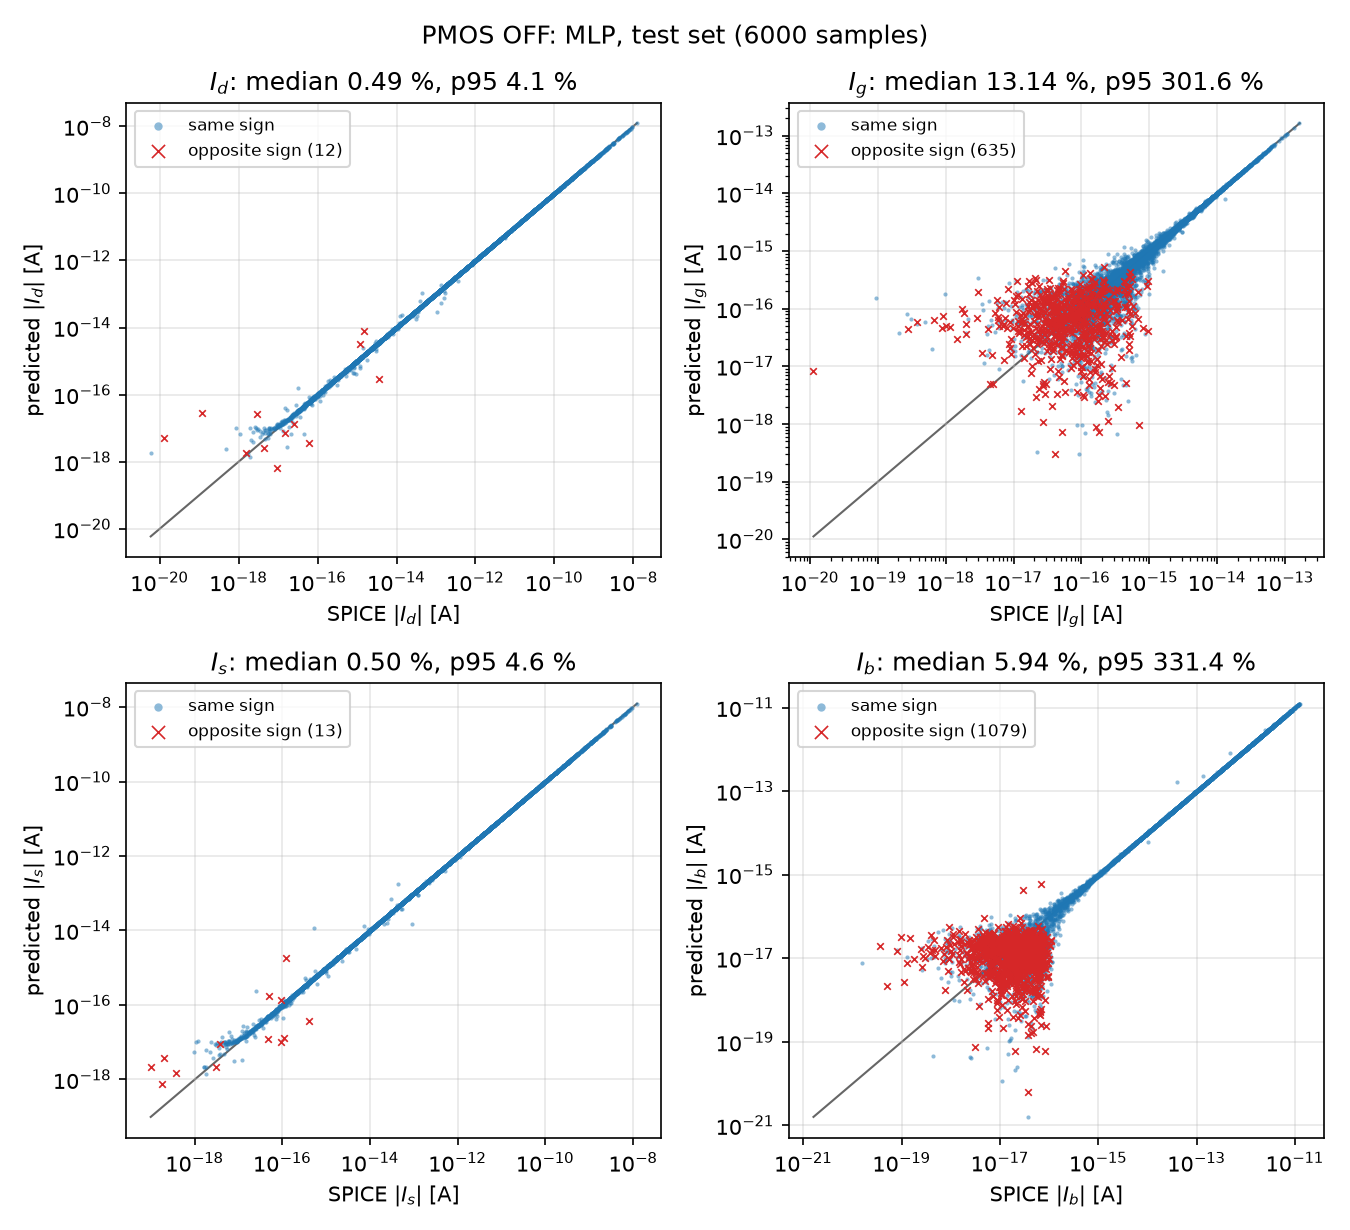
\includegraphics[width=\linewidth]{test_pred_vs_spice_pmos_off.png}\caption{PMOS OFF}\end{subfigure}
\caption{As Fig.~\ref{fig:testplots_n}, for the chosen PMOS models.}
\label{fig:testplots_p}
\end{figure}

\section{Gate results}\label{sec:gates}
\subsection{SPICE reference}
Each gate has a hand-written transistor-level netlist (\texttt{netlists/gates/<gate>.cir}) with the
transistor netlists' junction geometry and \texttt{.options} line. Widths are not set by the spec;
we use standard static-CMOS sizing in units of $L_{\min}$: INV $n=1$, $p=2$; NAND2 $n=p=2$; NOR2 $n=1$,
$p=4$; AND2 and OR2 are a NAND2 / NOR2 followed by an INV, simulated as one gate. Inputs are named
along each stack from the rail to the output: in the NAND2 (and AND2) NMOS stack $A$ drives the
transistor at ground and $B$ the one at the output (internal node $x$); in the NOR2 (and OR2) PMOS stack
$A$ drives the transistor at VDD and $B$ the one at the output (node $y$).
The 200 corners (\texttt{04\_gen\_corners.py}, seed 4242) each draw VDD, $T$, one set of NMOS and one
set of PMOS process parameters from the distributions of Section~4 of the spec. \texttt{05\_gate\_spice.py}
simulates all 18 gate/input cases at every corner (3{,}600 simulations) with the inputs at exactly 0 or
VDD and records the output and internal node voltages and every source current. The leakage is the
static power divided by VDD: the current delivered by the VDD supply plus the currents delivered by the
inputs held at VDD. Every output settled within $7.2\times10^{-4}\,V_{DD}$ of its logic value.

\subsection{ML prediction}
Following step~4 of the spec, \texttt{06\_gate\_preds.py} takes the terminal voltages of every
transistor from the SPICE node voltages of the same gate, inputs and corner (output, $x$, $y$ and the
NAND2/NOR2 output of AND2/OR2), the inputs, VDD and ground; the ML prediction therefore has no node
voltages of its own, and those recorded for it are the SPICE values. Each transistor runs through the
chosen model of its case (ON or OFF from the inputs). With every current flowing into its terminal, the
leakage is the sum of the currents into the terminals on VDD and on the inputs held at VDD, the same
definition as in SPICE.

\textbf{ON transistors via Kirchhoff's law.} In a static gate an ON transistor carries only what the
OFF transistors leak, with a few \si{\micro V} across it, so its predicted channel current would only
turn that tiny SPICE voltage drop into a current. We keep the ON transistors' predicted $I_g$ and $I_b$
but take their $I_d$ and $I_s$ from Kirchhoff's current law at the output and internal nodes. The
leakage is then set by the OFF transistor models and the gate and body currents.
Table~\ref{tab:gatemethods} compares this with two alternatives, also with the output-type nodes set to
exactly 0 or VDD: the ON models' own $I_d$/$I_s$ are slightly more accurate with the SPICE voltages but
collapse with ideal ones, i.e.\ their accuracy comes from the \si{\micro V} drops computed by SPICE, not
from the models.

\begin{table}[!htbp]
\centering
\caption{Gate leakage method, all 3{,}600 rows: median error and mean accuracy.}
\label{tab:gatemethods}
\small
\begin{tabular}{lccc}
\toprule
 & Kirchhoff for ON & ON models' & \\
 & (used) & $I_d$/$I_s$ & $\sum V I / V_{DD}$ \\
\midrule
Median error, SPICE node voltages & 1.40\,\% & 1.26\,\% & 1.69\,\% \\
Mean accuracy, SPICE node voltages & 97.4\,\% & 97.6\,\% & 96.4\,\% \\
Mean accuracy, ideal 0/VDD outputs & 97.4\,\% & 56.4\,\% & 97.0\,\% \\
\bottomrule
\end{tabular}
\end{table}

\textbf{OFF transistors at $|V_{ds}| \approx 0$.} An OFF transistor with both ends on the same rail (the
OFF PMOS of NAND2 01/10, the OFF NMOS of NOR2 01/10 and the corresponding AND2/OR2 cases; 1{,}600 of
the 3{,}600 rows) sits at $|V_{ds}| \approx 0.1$--\SI{600}{\micro V}. The OFF training data barely covers
this (24 of 10{,}000 PMOS OFF samples below 1\,mV), and there the networks extrapolate to unphysical
currents (up to \SI{e265}{A}). Such a transistor is therefore evaluated at $|V_{ds}| = 1$\,mV, where the
training data starts to be populated. The choice is set by the training-data coverage, not by the gate
SPICE results. Its effect is small: NAND2 01 and 10, where the floored transistor is an OFF PMOS, are
among the most accurate cases (median 0.31 and 0.55\,\%). As a sensitivity check, a 0.1\,mV floor leaves
every case median unchanged but lets single NAND2/AND2 corners reach 105\,\% error.

\subsection{Results}
Table~\ref{tab:gates} lists the 18 cases and Fig.~\ref{fig:gateparity} the parity plot. Over all 3{,}600
simulations the median error is 1.40\,\% (p95 9.4\,\%, maximum 29\,\%), the median bias $-0.6$\,\% and
the mean accuracy 97.4\,\%, against the target of 99\,\%. Per gate the median error is 0.5--2.1\,\% and
the mean accuracy 96.6--98.3\,\%.

\begin{table}[!htbp]
\centering
\caption{Gate leakage, ML vs SPICE, 200 corners per case. Bias: median of (ML$-$SPICE)/SPICE;
error: $|$ML$-$SPICE$|$/SPICE; mean accuracy: $100\,\% - $ mean error.}
\label{tab:gates}
\small
\begin{tabular}{llrrrrrr}
\toprule
 & & \multicolumn{2}{c}{Median leakage (nA)} & Bias & \multicolumn{2}{c}{Error (\%)} & Mean acc. \\
\cmidrule(lr){3-4}\cmidrule(lr){6-7}
Gate & $AB$ & SPICE & ML & (\%) & median & p95 & (\%) \\
\midrule
INV & 0 & 1.603 & 1.597 & $-$0.34 & 1.07 & 4.2 & 98.6 \\
INV & 1 & 1.424 & 1.348 & $-$3.04 & 4.04 & 14.9 & 94.5 \\
\midrule
NAND2 & 00 & 0.132 & 0.131 & $-$0.03 & 0.24 & 0.8 & 99.7 \\
NAND2 & 01 & 1.231 & 1.230 & +0.17 & 0.31 & 1.0 & 99.6 \\
NAND2 & 10 & 3.988 & 3.968 & +0.17 & 0.55 & 3.3 & 99.1 \\
NAND2 & 11 & 2.935 & 2.770 & $-$2.85 & 3.92 & 14.0 & 94.8 \\
\midrule
NOR2 & 00 & 3.206 & 3.200 & $-$0.33 & 1.06 & 4.2 & 98.6 \\
NOR2 & 01 & 3.108 & 2.934 & $-$2.83 & 3.37 & 12.1 & 95.3 \\
NOR2 & 10 & 0.670 & 0.658 & +0.81 & 2.24 & 6.7 & 97.3 \\
NOR2 & 11 & 0.082 & 0.083 & +0.24 & 1.27 & 6.1 & 98.1 \\
\midrule
AND2 & 00 & 1.728 & 1.615 & $-$2.61 & 3.47 & 13.2 & 95.2 \\
AND2 & 01 & 3.312 & 3.243 & $-$1.40 & 1.92 & 9.2 & 97.0 \\
AND2 & 10 & 6.451 & 6.402 & $-$0.63 & 1.20 & 6.3 & 98.0 \\
AND2 & 11 & 5.262 & 5.104 & $-$2.17 & 2.62 & 10.5 & 96.4 \\
\midrule
OR2 & 00 & 5.489 & 5.435 & $-$1.66 & 1.83 & 7.4 & 97.4 \\
OR2 & 01 & 5.587 & 5.513 & $-$1.99 & 2.36 & 9.5 & 96.7 \\
OR2 & 10 & 2.822 & 2.741 & $-$0.31 & 1.14 & 3.9 & 98.5 \\
OR2 & 11 & 1.659 & 1.648 & $-$0.29 & 1.00 & 4.0 & 98.7 \\
\bottomrule
\end{tabular}
\end{table}

\begin{figure}[!htbp]
\centering
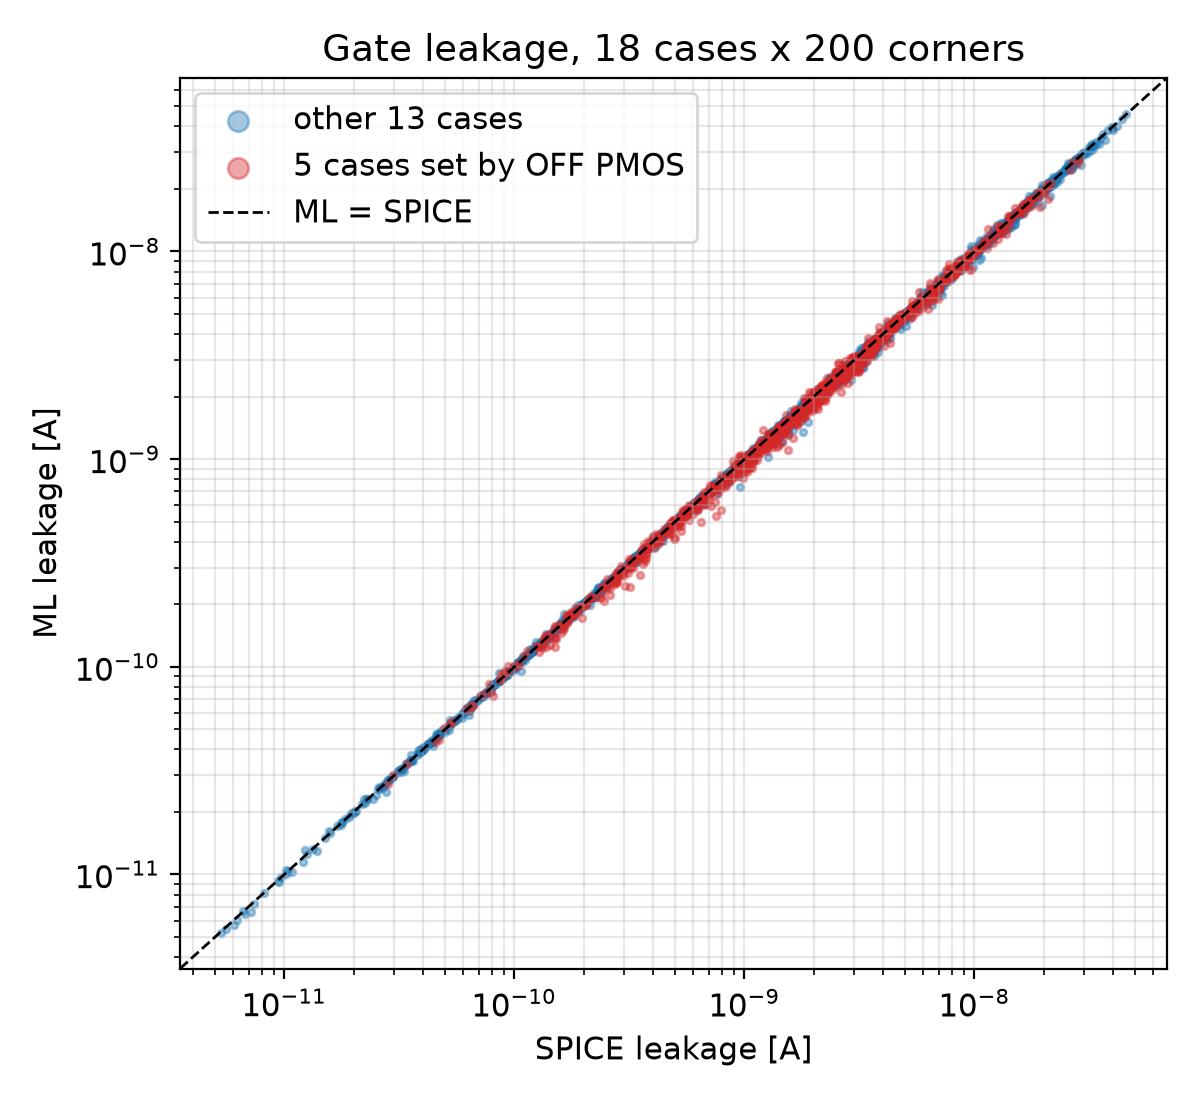
\includegraphics[width=0.6\linewidth]{gate_parity_by_case.png}
\caption{ML vs SPICE gate leakage, all 18 cases $\times$ 200 corners, log axes; red: the five cases
whose leakage is set by OFF PMOS transistors.}
\label{fig:gateparity}
\end{figure}

\textbf{Most and least accurate.} The accuracy of a case follows how much of its leakage is set by the
PMOS OFF model. In the five least accurate cases, INV 1, NAND2 11, AND2 00, NOR2 01 and NOR2 10, 89--99\,\%
of the leakage is OFF-PMOS current (measured as the change of the predicted leakage when the PMOS OFF
currents are scaled); together they have a median error of 3.2\,\% and a mean accuracy of 95.4\,\%,
and the first four are biased low by 2.6--3.0\,\%. The other 13 cases have a median error of 1.0\,\% and
a mean accuracy of 98.2\,\%; NAND2 00, 01 and 10, carried by the NMOS OFF model, are the most accurate
(0.24--0.55\,\%).

\section{Test-circuit results}\label{sec:circuit}
\paragraph{Circuit.} The 8-bit parity checker (\texttt{netlists/circuit/parity8.cir}) is built only
from a gate that has ML models: 28 NAND2, 112 transistors. Each XOR2 is four NAND2 gates,
$a \oplus b = \overline{\overline{a\,n_1}\cdot\overline{b\,n_1}}$ with $n_1 = \overline{ab}$; seven XOR2
form a balanced three-level tree, giving $out = in_0 \oplus \dots \oplus in_7$. Transistor widths,
junction geometry and pin order are those of the NAND2 gate netlist, with the spec's \texttt{.options}
line. The gate list used by the ML prediction (\texttt{data/circuit/gates.csv}) is read from the netlist
itself, so the two cannot differ.

\paragraph{SPICE reference.} \texttt{07\_circuit\_spice.py} simulates all 256 input vectors at the same
200 corners as the gates (51{,}200 simulations), with the leakage defined as for the gates. Every output
was within $8\times10^{-4}\,V_{DD}$ of its logic value and every leakage positive; the median leakage per
vector ranges from \SI{48}{nA} to \SI{97}{nA}.

\paragraph{Hierarchical ML prediction.} \texttt{08\_circuit\_ml.py} derives, for each input vector, the
logic value of every net and so the input combination of each NAND2. Every circuit corner is a gate
corner, so the ML leakage of a gate is its gate-level prediction for that input combination and corner,
and the circuit leakage is the sum over the 28 gates (spec step 7). The same sum of the gate SPICE
leakages isolates the hierarchical assumptions (inputs at exactly 0 or VDD, no loading).

\begin{table}[!htbp]
\centering
\caption{Test-circuit leakage vs circuit SPICE, 256 input vectors $\times$ 200 corners, with the
metrics of Table~\ref{tab:gates}. The gate SPICE sum is the same composition with the gate SPICE
leakages; the gate rows are the gate-level reference.}
\label{tab:circuit}
\resizebox{\linewidth}{!}{%
\begin{tabular}{lrrrrrrrr}
\toprule
Estimate & Rows & SPICE med. (nA) & Est.\ med. (nA) & Bias (\%) & Med.\ err.\ (\%) & p95 (\%) & Mean acc.\ (\%) & Max (\%) \\
\midrule
ML sum of gate predictions & 51{,}200 & 79.92 & 78.47 & $-$0.91 & 1.36 & 7.6 & 97.6 & 22.3 \\
Gate SPICE sum (no ML)     & 51{,}200 & 79.92 & 79.91 & $-$0.04 & 0.04 & 0.21 & 99.9 & 0.51 \\
\midrule
Gates, NAND2 cases         & 800      & 1.429 & 1.426 & $-$0.03 & 0.48 & 8.9 & 98.3 & 28.5 \\
Gates, all 18 cases        & 3{,}600  & 2.128 & 2.097 & $-$0.56 & 1.40 & 9.4 & 97.4 & 29.4 \\
\bottomrule
\end{tabular}}
\end{table}

\begin{figure}[!htbp]
\centering
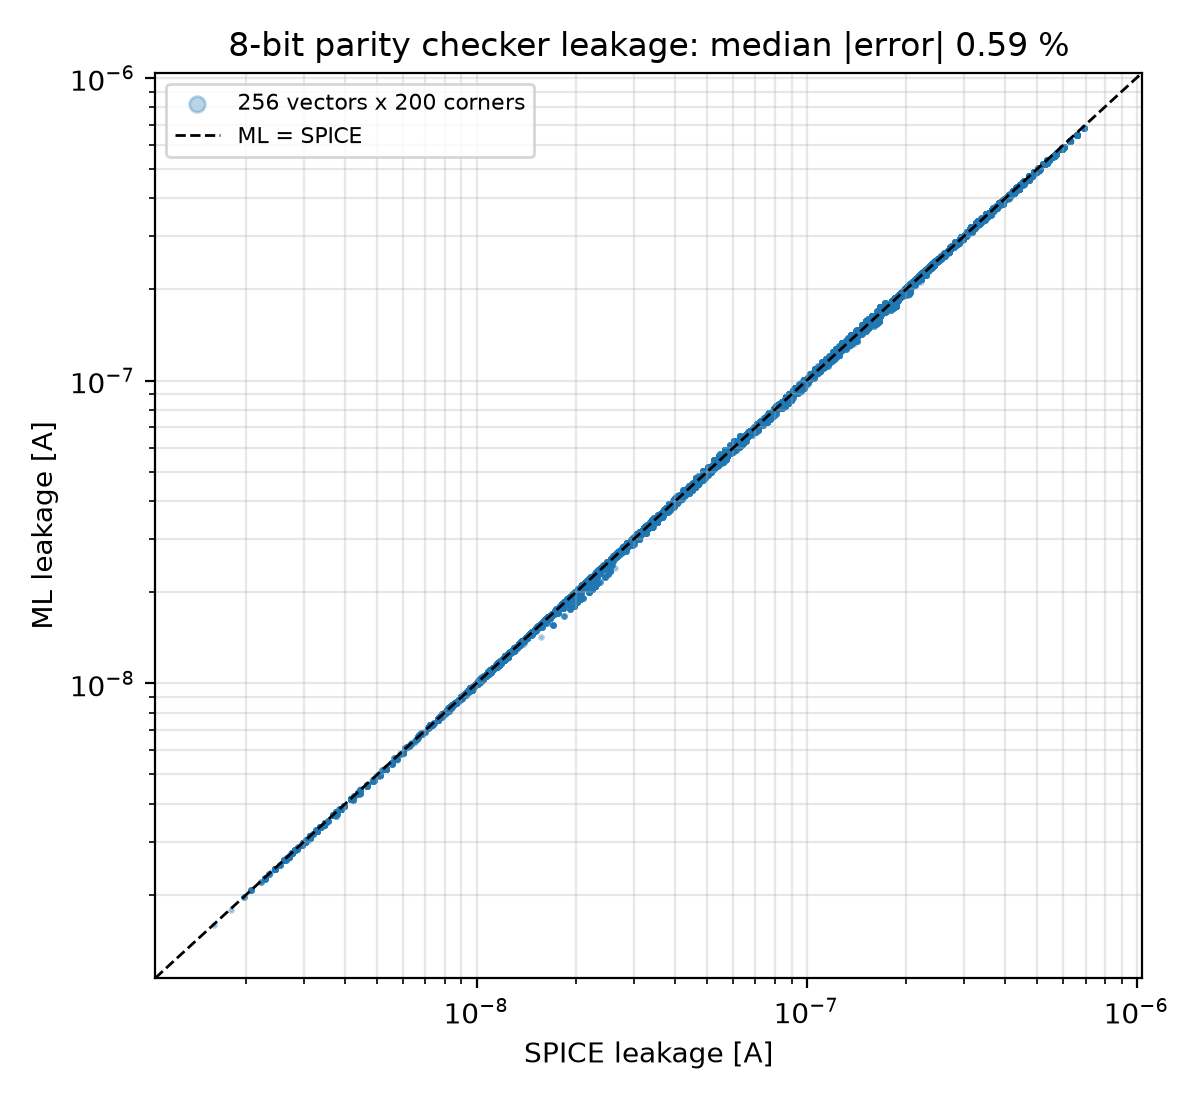
\includegraphics[width=0.6\linewidth]{circuit_parity.png}
\caption{ML vs SPICE leakage of the 8-bit parity checker, all 256 input vectors $\times$ 200 corners, log axes.}
\label{fig:circuitparity}
\end{figure}

\paragraph{Comparison with the gates.} Table~\ref{tab:circuit} and Fig.~\ref{fig:circuitparity} give the
result. The hierarchical assumptions cost only 0.04\,\% median error (gate SPICE sum), so the circuit
error is the gate-level ML error carried over. Per input vector (\texttt{results/circuit\_results\_per\_vector.csv},
200 corners each) the median error is 1.27--1.82\,\%, the p95 6.6--9.0\,\% and the mean accuracy
97.1--97.7\,\%. The circuit (1.36\,\%) is less accurate than the pooled NAND2 cases (0.48\,\%) because
it weights the input combinations by leakage: every vector has 7 to 11 gates at 11 (two OFF PMOS, median
error 3.9\,\%, bias $-2.85\,\%$), and they carry a median 39\,\% of the circuit leakage.
At each vector and corner the circuit error is the leakage-weighted average of the gate errors plus the
composition error ($\le 0.51\,\%$). Gates at the same input combination and corner have the same error,
so it does not average out over more gates. Keeping only the errors of the gates at 11 (all other gates
at their SPICE leakage) gives 1.36\,\% median and $-1.09\,\%$ bias, the full result; keeping only those
of 00, 01 and 10 gives 0.24\,\% and $+0.01\,\%$. The circuit error is therefore that of its OFF-PMOS
gates. The maximum, $-22.3\,\%$ at corner 152, is the NAND2 11 error there ($-28.5\,\%$) weighted by the
78\,\% leakage share of those gates.

\section{Error analysis}\label{sec:errors}
\paragraph{Transistor level: the PMOS OFF drain current.} Gate and circuit leakage are carried by the
OFF transistors' $I_d$, so the PMOS OFF $I_d$ error (test median 3.0\,\% against 0.14\,\% for NMOS OFF)
is what limits every level above. Figure~\ref{fig:offid} shows that this is not mainly a noise-floor
effect. Below about \SI{1e-14}{A} both OFF models lose accuracy, as expected at the \SI{1e-15}{A} floor
(20\,\% of the PMOS OFF $I_d$ values are below it). From about \SI{1e-12}{A} up, the NMOS OFF error is
0.1--0.25\,\%, but the PMOS OFF error stays at 1.5--2\,\% up to \SI{1e-8}{A} (1.8\,\% median for $|I_d| \ge \SI{1e-12}{A}$,
against 0.12\,\%), and it is 10--30 times the NMOS OFF error at every temperature, rising from about
1.7\,\% at \SI{115}{\celsius} to 6\,\% at \SI{-30}{\celsius}. At the currents that matter for gate
leakage (nA) the PMOS OFF error is therefore a model limitation. The most likely causes are that one
network learns all four PMOS OFF currents, two of which ($I_g$ and, in half the rows, $I_b$) are mostly
noise-floor labels with near-random sign that compete with $I_d$ for capacity and loss, and that the
smallest PMOS OFF currents, at low temperature, sit close to the floor; a separate $I_d$/$I_s$ network
for PMOS OFF would test the first cause directly. $I_g$ and $I_b$ themselves (14.3 and 12.0\,\% median
for PMOS OFF) are limited by the noise floor but are negligible in the gate sums.

\begin{figure}[!htbp]
\centering
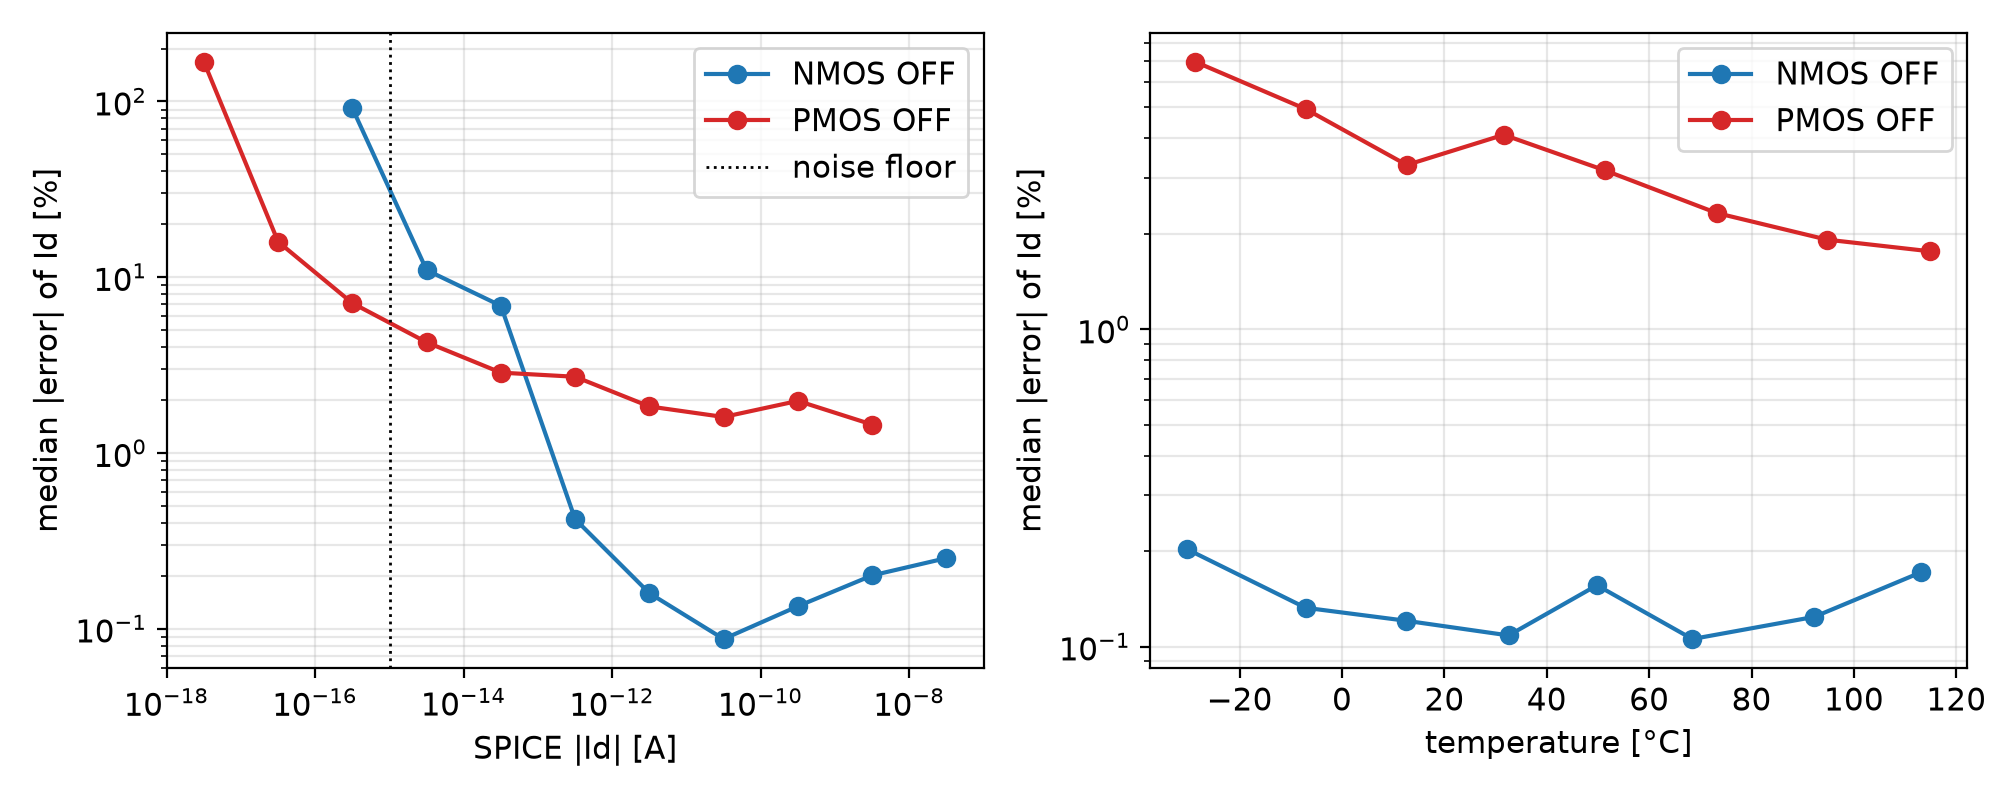
\includegraphics[width=0.9\linewidth]{off_id_error.png}
\caption{Test-set median error of the OFF-case $I_d$ (chosen MLPs), against the SPICE $|I_d|$ (decade
bins) and against temperature (8 quantile bins). Dotted line: simulator noise floor.}
\label{fig:offid}
\end{figure}

\paragraph{Gate level.} The largest gate errors are in the five cases set by OFF PMOS transistors
(Section~\ref{sec:gates}). Temperature matters most for the tails: the p95 error is 14.5\,\% for
$T \le \SI{0}{\celsius}$ and 5.9\,\% above \SI{80}{\celsius} (median 1.7 vs 1.1\,\%), and 35 of the worst
36 rows (1\,\%) are below \SI{0}{\celsius}, against 24\,\% of all rows. The median error rises from 1.2 to
1.8\,\% from the highest to the lowest quarter of PMOS $|v_{th0}|$ and from 1.0 to 2.0\,\% from the lowest
to the highest VDD quarter; NMOS $v_{th0}$ has little effect (1.3--1.5\,\%). Figure~\ref{fig:corner}
shows the same trends for the NAND2 11 case and the circuit.

\paragraph{Circuit level.} The corner, not the input vector, sets the circuit error: the corner explains
99.6\,\% of its variance, as expected when all 28 gates share one VDD, temperature and process draw. The
error rises with the OFF-PMOS share of the leakage, from 0.8\,\% median in its lowest quarter to 3.2\,\%
in its highest (\texttt{results/circuit\_error\_breakdown.csv}). Ranked with one point per corner
(Spearman, 200 corners; \texttt{results/circuit\_error\_drivers.csv}), PMOS $|v_{th0}|$ and temperature
are equally strong drivers ($r = -0.36$), then NMOS $v_{th0}$ ($+0.23$); VDD is weak ($+0.14$). The two
$v_{th0}$ act through the OFF-PMOS share (a low PMOS $|v_{th0}|$ or a high NMOS $v_{th0}$ raises it;
Spearman with the share $-0.70$ and $+0.72$), temperature through the NAND2 11 error itself (colder is
more negative, $r = +0.49$). This is why NMOS $v_{th0}$ matters for the circuit although it barely
affects any single gate. The worst 1\,\% of rows come from two corners, both among the three lowest
PMOS $|v_{th0}|$ (0.445\,V) and at $-28$ and \SI{-38}{\celsius}.

\begin{figure}[!htbp]
\centering
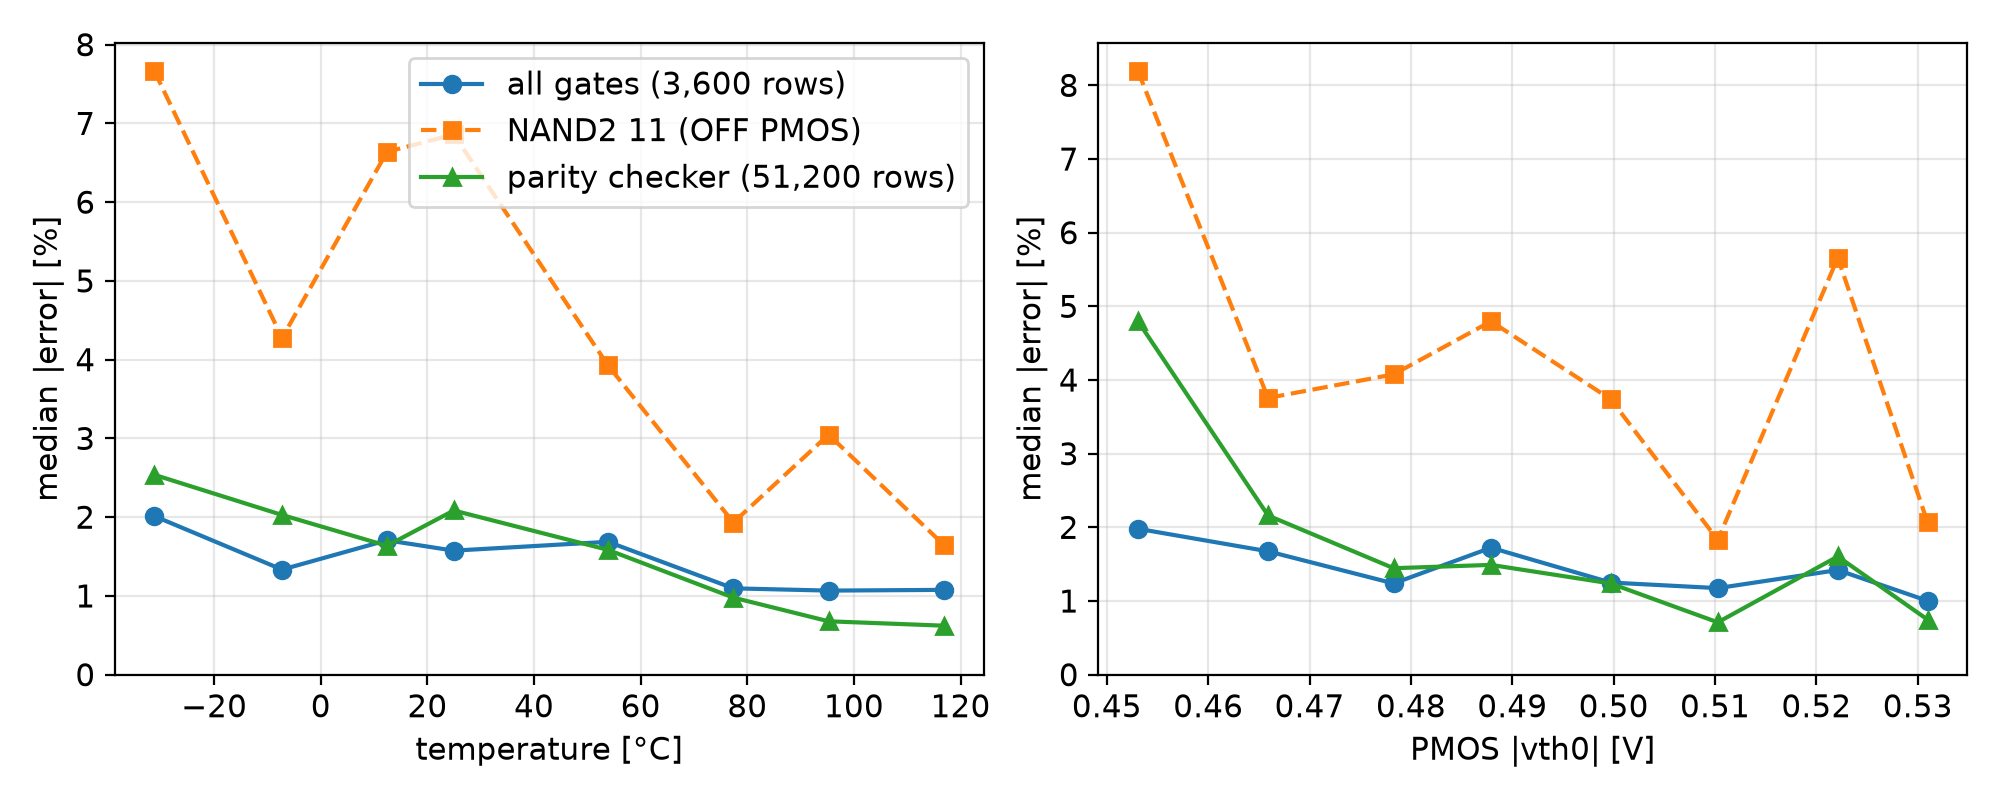
\includegraphics[width=0.9\linewidth]{error_vs_corner.png}
\caption{Median $|$error$|$ against temperature and PMOS $|v_{th0}|$ (8 quantile bins of the corners):
all gate rows, the NAND2 11 rows (25 per bin, hence noisy) and the parity checker.}
\label{fig:corner}
\end{figure}

\section{Limitations and improvements}\label{sec:limits}
In order of their effect on the result:
\begin{enumerate}[leftmargin=*]
  \item \textbf{The PMOS OFF drain-current model limits everything above it.} With the NAND2 11 gates
        at their SPICE leakage, the parity checker would have a median error of 0.23\,\% and a mean
        accuracy of 99.6\,\% (\texttt{09\_report\_figures.py}), above the 99\,\% target. Improvements, in
        the order we would try them: a separate PMOS OFF network for $I_d$/$I_s$ only, so the noise-floor
        $I_g$/$I_b$ labels cannot compete with it; an ensemble of seeds (with the earlier targets, five
        MLPs halved the median error, e.g.\ PMOS OFF 12.0 to 8.8\,\%); and more PMOS OFF samples at low
        temperature and low $|v_{th0}|$, where its error is largest.
  \item \textbf{Not SPICE-free.} As spec step 4 prescribes, the gate prediction uses the gate SPICE node
        voltages of the same corner, so the estimate exists only at the 200 simulated corners. With
        Kirchhoff's law for the ON transistors the output-type nodes are not needed (Table~\ref{tab:gatemethods});
        solving the stack nodes $x$ and $y$ from the transistor models as well would remove the dependence.
  \item \textbf{OFF transistors at $|V_{ds}| \approx 0$} are evaluated at 1\,mV because the OFF datasets
        contain almost no samples there. Adding OFF samples with $|V_d - V_s|$ down to \SI{0.1}{\micro V}
        would remove this workaround.
  \item \textbf{Hierarchical assumptions} (exact 0/VDD gate inputs, no loading) cost 0.04\,\% for the
        parity checker. It uses one gate type with a fan-out of at most two, so it does not test higher
        fan-out or unlike loads, where the loading error may be larger.
  \item \textbf{Simulator noise floor.} Currents below \SI{1e-15}{A} are not reproducible with the
        unmodified card. This caps the PMOS OFF $I_g$/$I_b$ accuracy, but these currents are negligible
        in the gate sums.
  \item \textbf{Methodology caveats.} The test set was scored twice, once with the earlier asinh
        targets and once with the present ones; the change was decided on the validation set only.
        Several per-case target choices are within seed variation (Appendix~\ref{app:tt}). The
        hyperparameter search was manual and is not re-run by the final scripts. No learning curve was
        run, so we cannot say how much smaller than 10{,}000 samples per case would suffice.
\end{enumerate}

\section{Conclusion}
A hierarchical ML model built from four MLP transistor models predicts the leakage of five gates and of
an 8-bit parity checker under PVT variation with a median error of 1.4\,\% and a mean accuracy of
97.4--97.6\,\%, against SPICE at 200 corners. Three of the four transistor models are accurate to about
0.15\,\%, and composing gates into the circuit costs only 0.04\,\%. The remaining error, and the gap to
the 99\,\% target, comes from one source: the drain current of the PMOS OFF model, which a dedicated
model or more targeted data should close.

\begin{thebibliography}{9}
\bibitem{roy2003} K.~Roy, S.~Mukhopadhyay and H.~Mahmoodi-Meimand, ``Leakage current mechanisms and
  leakage reduction techniques in deep-submicrometer CMOS circuits,'' \emph{Proc.\ IEEE}, vol.~91,
  no.~2, pp.~305--327, 2003.
\bibitem{ptm} Predictive Technology Model (PTM), Arizona State University, \url{https://ptm.asu.edu}.
\bibitem{bsim4} BSIM Group, \emph{BSIM4 MOSFET Model User's Manual}, University of California, Berkeley.
\bibitem{ngspice} H.~Vogt et al., \emph{Ngspice User's Manual}, version~47, \url{https://ngspice.sourceforge.io}.
\bibitem{ekv} C.~C.~Enz, F.~Krummenacher and E.~A.~Vittoz, ``An analytical MOS transistor model valid
  in all regions of operation and dedicated to low-voltage and low-current applications,''
  \emph{Analog Integr.\ Circuits Signal Process.}, vol.~8, pp.~83--114, 1995.
\bibitem{pytorch} A.~Paszke et al., ``PyTorch: an imperative style, high-performance deep learning
  library,'' \emph{NeurIPS}, 2019.
\bibitem{sklearn} F.~Pedregosa et al., ``Scikit-learn: machine learning in Python,'' \emph{J.\ Mach.\
  Learn.\ Res.}, vol.~12, pp.~2825--2830, 2011.
\bibitem{xgboost} T.~Chen and C.~Guestrin, ``XGBoost: a scalable tree boosting system,'' \emph{KDD}, 2016.
\end{thebibliography}

\appendix
\section{MLP hyperparameter search}
\label{app:mlp}
Values are the validation mean of the four median errors, with the earlier target
$\operatorname{asinh}(I/\SI{1e-18}{A})$ (before the study of Appendix~\ref{app:tt}).

\begin{table}[!htbp]
\centering
\small
\caption{Round 1 (base: $128\times3$, SiLU, MSE, peak LR $3\times10^{-3}$, batch 256, 3,000 epochs; one change per row).}
\begin{tabular}{llcc}
\toprule
\# & Change from base & NMOS ON & PMOS OFF \\
\midrule
1 & none                      & 1.54\,\% & 24.20\,\% \\
2 & $256\times4$              & 2.09\,\% & 21.51\,\% \\
3 & L1 loss                   & \textbf{0.87\,\%} & 18.32\,\% \\
4 & Huber loss                & 1.35\,\% & 20.21\,\% \\
5 & $256\times4$ + L1 loss    & 1.10\,\% & \textbf{12.56\,\%} \\
6 & tanh                      & 2.31\,\% & 56.25\,\% \\
7 & $256\times4$ + GELU       & 1.88\,\% & 25.00\,\% \\
8 & $256\times4$ + peak LR 0.01 & 2.84\,\% & 30.05\,\% \\
\bottomrule
\end{tabular}
\end{table}

\begin{table}[!htbp]
\centering
\small
\caption{Round 2 (all L1 loss, SiLU, peak LR $3\times10^{-3}$).}
\begin{tabular}{llcccc}
\toprule
 & Setting & NMOS ON & NMOS OFF & PMOS ON & PMOS OFF \\
\midrule
A & $128\times3$, 3,000 epochs          & 0.87\,\% & 0.81\,\% & 0.91\,\% & 18.32\,\% \\
B & $256\times4$, 3,000 epochs          & 1.10\,\% & 0.60\,\% & 0.92\,\% & 12.56\,\% \\
C & $128\times3$, 6,000 epochs          & \textbf{0.71\,\%} & 0.58\,\% & \textbf{0.71\,\%} & 15.66\,\% \\
D & $256\times4$, weight decay $10^{-3}$ & 1.00\,\% & \textbf{0.57\,\%} & 0.90\,\% & \textbf{12.00\,\%} \\
E & $128\times3$, batch 128             & 0.72\,\% & 0.62\,\% & 0.73\,\% & 14.37\,\% \\
\bottomrule
\end{tabular}
\end{table}

\section{Target-transform study}
\label{app:tt}
The optional script \texttt{experiments/\allowbreak target\_transforms.py} (about 1.5--2.5\,h) writes the
full tables to \texttt{results/\allowbreak experiments/\allowbreak transforms\_tables.md}. It uses the
validation set only; the test rows are never loaded. Each transform builds on the previous one unless noted:
\begin{itemize}[itemsep=1pt]
  \item \textbf{asinh}: the earlier target $\operatorname{asinh}(I/\SI{1e-18}{A})$ (seed 42 only).
  \item \textbf{T0}: $\log_{10}|I|$ plus a sign output per current with mixed training signs.
  \item \textbf{T1}: canonical drain/source swap; $I_d$ sign from physics, $I_s$, $I_g$, $I_b$ keep the sign output.
  \item \textbf{T2}: per-width target $\log_{10}(|I|/W)$.
  \item \textbf{T3a}: T2 plus the inputs $V_{ds}/V_T$, $V_{gs}/V_T$, $V_{bs}/V_T$, $\log_{10}(1-e^{-|V_{ds}|/V_T}+10^{-12})$.
  \item \textbf{T3b}: T2 with the $I_d$/$I_s$ target $\log_{10}\bigl(|I|/(W(1-e^{-|V_{ds}|/V_T})+10^{-30})\bigr)$.
  \item \textbf{T4}: best of T0--T3b with $I_s = -(I_d+I_g+I_b)$ instead of predicting $I_s$.
  \item \textbf{T5}: best of T0--T4 with training labels clipped to $|I| \ge \SI{1e-17}{A}$.
\end{itemize}
The MLP and XGBoost were trained with seeds 42, 43 and 44; ``best'' and the final choice use the rule
of Section~\ref{sec:choice} on the mean over the three seeds. XGBoost did not improve on its own design
with any transform. Within seed variation (mean $\pm$ standard deviation of the mean median error):
\begin{itemize}[itemsep=1pt]
  \item NMOS OFF: T4 on T3a (0.136 $\pm$ 0.003\,\%) is clearly ahead of T3a (0.229 $\pm$ 0.007\,\%).
  \item NMOS ON: T3b (0.157 $\pm$ 0.004\,\%) against T3a (0.162 $\pm$ 0.010\,\%): within seed variation.
  \item PMOS ON: T3b (0.152 $\pm$ 0.003\,\%) against T3a (0.152 $\pm$ 0.007\,\%): a tie.
  \item PMOS OFF: T5 on T3a (8.19 $\pm$ 0.06\,\%) against T3a (8.46 $\pm$ 0.22\,\%): within seed variation.
\end{itemize}
The step from the asinh target to the log targets with the drain/source swap (T1 onwards) is far larger
than the seed variation in every case. With the asinh target, most of the largest ON-case $I_d$/$I_s$
errors were at $|V_d - V_s| < \SI{20}{mV}$, where the channel current changes sign (median 7.6\,\% there);
the swap, the sign output and the saturation-factor target bring this to 0.4--0.5\,\%. Clipping (T5)
changes nothing for the ON cases and ruins NMOS OFF $I_b$ (p95 about 1{,}400\,\%), whose values are
genuinely \SIrange{1e-19}{1e-17}{A}.

\section{Details of the other model types}
\label{app:models}
\paragraph{Polynomial ridge.} A global polynomial of the raw inputs fails on $I_d$ and $I_s$ (about
100\,\% median error at degree 2--4) because they change sign with $V_d-V_s$. The model predicts
$D/V_{ds}$ with $D = I_d - I_s$ (even in $V_{ds}$ and positive in all 40{,}000 samples), $I_g$ and $I_b$
(log magnitude with the majority training sign), each with its own ridge regression; then
$I_d = (D - I_g - I_b)/2$ and $I_s = (-D - I_g - I_b)/2$. Features: PMOS voltages mirrored
($V \to V_{DD} - V$) and drain/source sorted into $V_{lo}$, $V_{hi}$; base features $V_{DD}$, $V_{lo}$,
$V_{hi}$, $1/T$, $\ln W$ and the process parameters; the subthreshold drain factor
$\ln[(1-e^{-V_{ds}/V_T})/(V_{ds}/V_T)]$; EKV inversion charges $\ln q$,
$q=\ln(1+e^{(V_G - V - |v_{th0}|)/2nV_T})$ at each end and $\ln[(q_{lo}^2-q_{hi}^2)V_T/V_{ds}]$; a sharper
softplus and $t_{oxe}(V_G - V)$ at each end for gate tunnelling; $E_g(T)/V_T$ and an optional junction
reverse-bias factor. Pipeline: standardise, \texttt{PolynomialFeatures}, standardise, \texttt{Ridge}.
Degree $\in\{2,3,4\}$, $\alpha \in \{10^{-7},\dots,1\}$; selecting on the median error instead of the
log RMSE picked fits that predicted up to \SI{1e130}{A} at sparse validation points. The EKV charges took
the ON-case $I_d$ error from about 4\,\% to 0.7\,\%. Settings: \texttt{results/poly\_ridge\_validation.csv}.

\paragraph{XGBoost.} The model predicts $I_{ch} = (I_d - I_s)/2 \cdot \operatorname{sign}(V_d - V_s)$,
$I_{cm} = (I_d + I_s)/2$, $I_g$ and $I_b$, each as $\operatorname{asinh}\bigl(I / (\SI{1e-18}{A}\cdot W/L_{\min})\bigr)$.
Features (31): the inputs other than $V_d$, $V_s$; $1/T$; $V_{lo}$, $V_{hi}$, their gap and
$\ln(1 - e^{-(V_{hi}-V_{lo})/V_T})$; $V_g - V$ and $V_b - V$ at each end, also divided by $V_T$ and by
$t_{oxe}$; $\ln W$, $\ln t_{oxe}$, $\ln N_{dep}$, $\ln u_0$ and $v_{th0}/V_T$. Each booster starts from a
least-squares line (\texttt{base\_margin}). Settings: 6{,}000 rounds, learning rate 0.015, depth 6, row
and column subsampling 0.8, seed 42, 2 threads; min.\ child weight 5 and $\lambda = 5$ (PMOS OFF: L1
loss, 1 and 1). Version pinned (3.2.0); results can differ slightly between machines.

\paragraph{Random forest.} Inputs: $V_{DD}$, $T$, $W$, $V_{gs}$, $V_{ds}$, $V_{bs}$ and the five process
parameters. Tuned one at a time on the mean validation $R^2$: \texttt{max\_features} $\in\{3, 4, 6, 0.5, 1.0\}$,
\texttt{n\_estimators} $\in\{10, 50, 100, 200\}$, \texttt{max\_depth} $\in\{8, 12, 16, 20, \text{none}\}$,
\texttt{min\_samples\_leaf} $\in\{1, 2, 5, 10\}$; seed 2026. Chosen: 200 trees; depth 12 / none / 20 / 12,
\texttt{max\_features} 1.0 / 6 / 6 / 0.5, \texttt{min\_samples\_leaf} 1 / 1 / 1 / 5 (NMOS ON / NMOS OFF /
PMOS ON / PMOS OFF). The tuning $R^2$ stays above 0.9 for $I_d$, $I_s$ even at 35--91\,\% median error,
which shows why $R^2$ on a log scale is not a useful selection metric here.

\end{document}
